%lab report 3 of midpoint ellipse drawing algorithm
\documentclass[12pt]{article}

\usepackage{amsmath}
\usepackage{graphicx}
\usepackage[a4paper]{geometry}

\geometry{
  textwidth=\dimexpr\paperwidth-29mm,
  textheight=\dimexpr\paperheight-32mm,
  noheadfoot,
  nomarginpar
}

\setlength{\topskip}{0mm}
\setlength{\parindent}{0mm}

\begin{document}
	\title{Midpoint Ellipse}
	\author{Jenish Pant}
	\date{\today}
	\maketitle

	\section{Objective}
	To draw an ellipse using midpoint ellipse drawing algorithm.
	\section{Theory}
	
	\subsection{Midpoint Ellipse Drawing Algorithm}
	The midpoint ellipse algorithm is an algorithm used to determine the points needed for drawing an ellipse. It is a variant of Bresenham's circle algorithm where the calculation of \textit{d} is altered to accommodate for the ellipses' eccentricity.

	\section{Algorithm}
	\begin{enumerate}
		\item Input the center of the ellipse, radius in x and y direction.
		\item Calculate the initial value of the decision parameter in region 1 as $p_1 = b^2 - a^2b + \frac{1}{4}a^2$.
		\item At each $x_k$ position starting at k = 0, perform the following test:
		\begin{enumerate}
			\item If $p_k < 0$, the next point along the ellipse at $x_{k+1}$ is chosen to be $(x_k + 1, y_k)$ and $p_{k+1} = p_k + 2b^2x_{k+1} + b^2$.
			\item If $p_k \geq 0$, the next point along the ellipse at $x_{k+1}$ is chosen to be $(x_k + 1, y_k - 1)$ and $p_{k+1} = p_k + 2b^2x_{k+1} - 2a^2y_{k+1} + b^2$.
		\end{enumerate}
		\item Repeat step 3 until $2b^2x \geq 2a^2y$.
		\item At each yk position starting at k = 0, perform the following test:
		\begin{enumerate}
			\item If $p_k > 0$, the next point along the ellipse at $y_{k+1}$ is chosen to be $(x_k, y_k - 1)$ and $p_{k+1} = p_k - 2a^2y_{k+1} + a^2$.
			\item If $p_k \leq 0$, the next point along the ellipse at $y_{k+1}$ is chosen to be $(x_k + 1, y_k - 1)$ and $p_{k+1} = p_k + 2b^2x_{k+1} - 2a^2y_{k+1} + a^2$.
		\end{enumerate}
		\item Repeat step 5 until $y_{k+1} = 0$.
	\end{enumerate}

	\section{Source Code}
	\begin{verbatim}
	#include <graphics.h>
	#include <math.h>
	
	void midpointEllipse(int xc, int yc, int a, int b)
	{
	    int x, y, p;
	    x = 0;
	    y = b;
	
	    //initial decision parameter
	    p = b * b - a * a * b + a * a / 4;
	
	    while (2 * x * b * b < 2 * y * a * a)
	    {
	        putpixel(xc + x, yc + y, GREEN);
	        putpixel(xc - x, yc + y, GREEN);
	        putpixel(xc + x, yc - y, GREEN);
	        putpixel(xc - x, yc - y, GREEN);
	        if (p < 0)
	        {
	            x = x + 1;
	            p = p + 2 * b * b * x + b * b;
	        }
	        else
	        {
	            x = x + 1;
	            y = y - 1;
	            p = p + 2 * b * b * x - 2 * a * a * y + b * b;
	        }
	    }
	    p = b * b * (x + 0.5) * (x + 0.5) + a * a * (y - 1) * (y - 1) - a * a * b * b;
	    while (y >= 0)
	    {
	        putpixel(xc + x, yc + y, GREEN);
	        putpixel(xc - x, yc + y, GREEN);
	        putpixel(xc + x, yc - y, GREEN);
	        putpixel(xc - x, yc - y, GREEN);
	        if (p > 0)
	        {
	            y = y - 1;
	            p = p - 2 * a * a * y + a * a;
	        }
	        else
	        {
	            y = y - 1;
	            x = x + 1;
	            p = p + 2 * b * b * x - 2 * a * a * y + a * a;
	        }
	    }
	}

	\end{verbatim}
	\section{Output}

	\begin{figure}[!h]
		%move to the left
		\hspace*{-1cm}
		\centering
		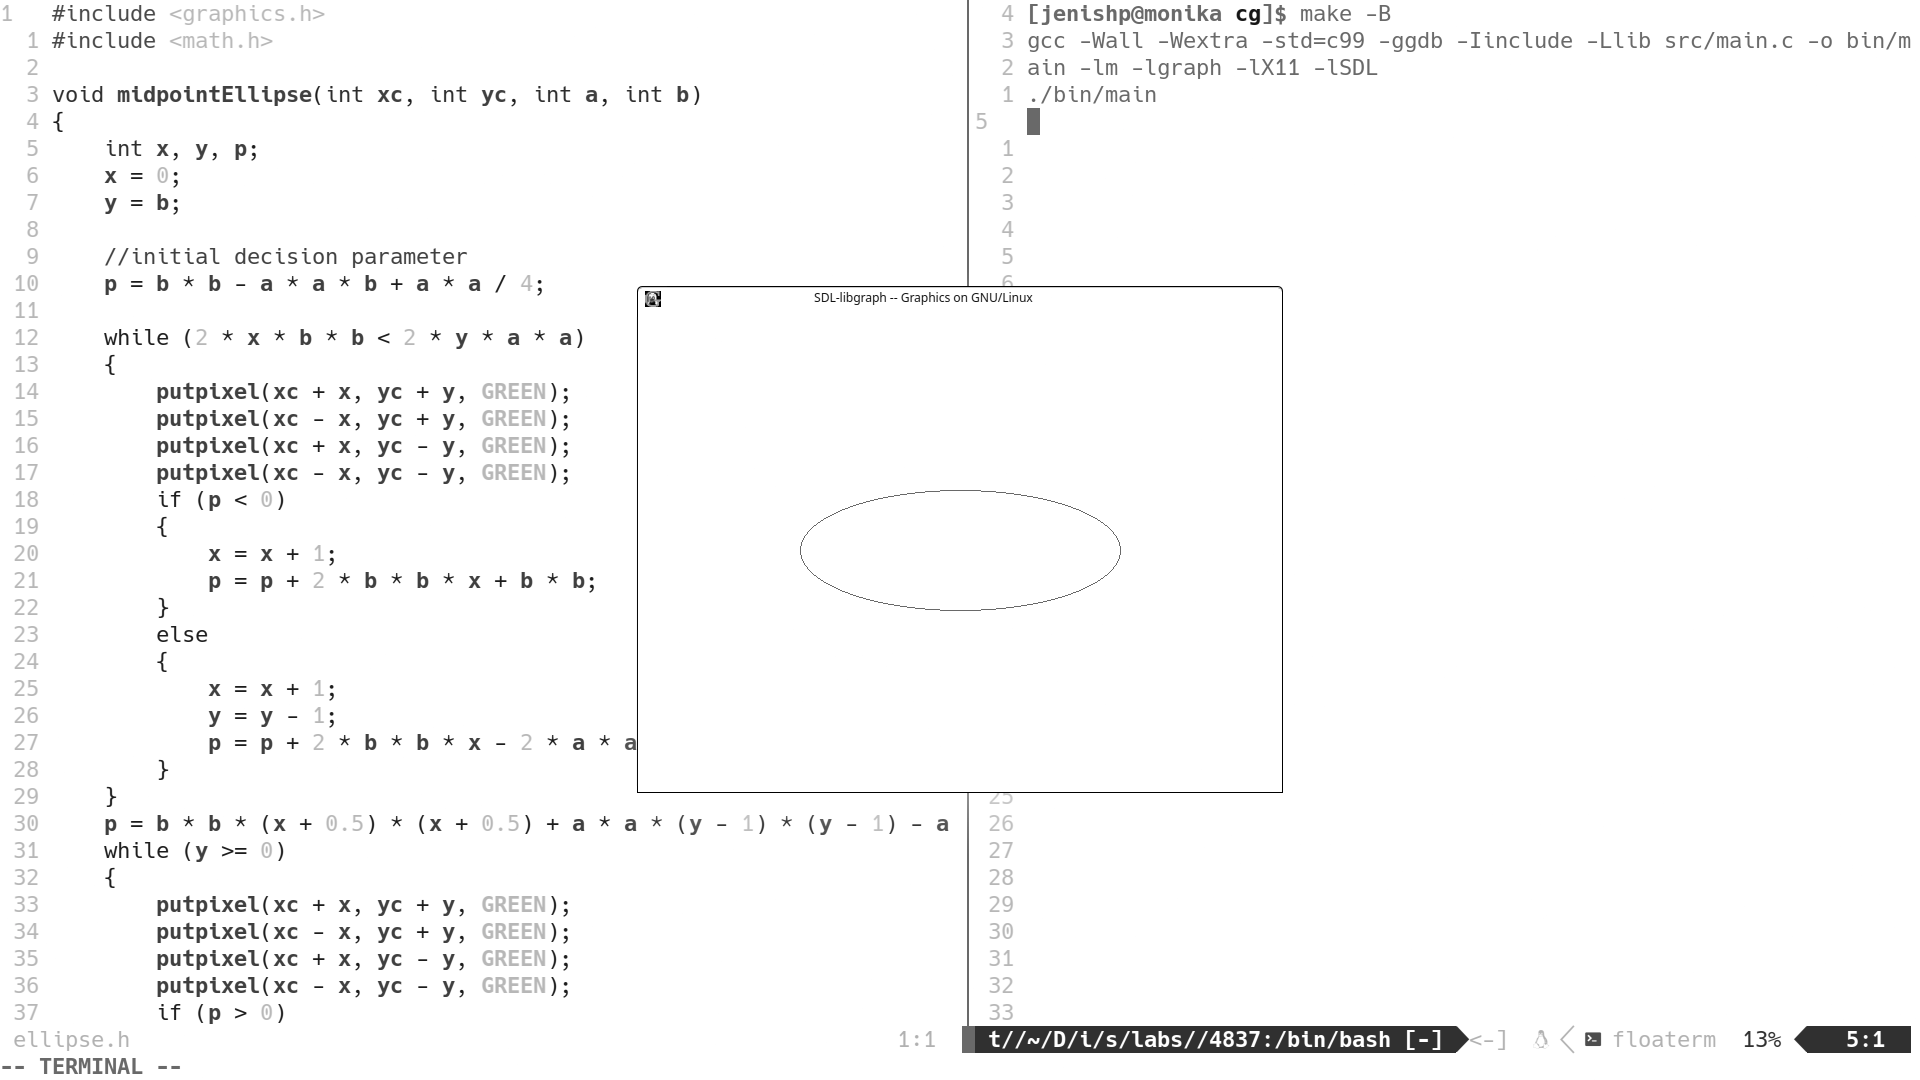
\includegraphics[width=1.01\linewidth]{output3.png}
		\caption{}
		\label{fig:}
	\end{figure}

	\section{Conclusion}
	We have successfully drawn an ellipse using midpoint ellipse drawing algorithm.

\end{document}

